\renewcommand{\NomeBloco}{current\_mirror\_nmos}
\renewcommand{\NomeBlocoNoUnderline}{curmirnmosb}
\renewcommand{\NomePTab}{tab_\NomeBlocoNoUnderline}
\renewcommand{\NomeSTab}{tab_\NomeBlocoNoUnderline2}
\renewcommand{\NomePFig}{fig_\NomeBlocoNoUnderline}
\renewcommand{\NomeSFig}{fig_\NomeBlocoNoUnderline2}
\renewcommand{\NomeTTab}{tab_\NomeBlocoNoUnderline3}
\renewcommand{\NomeQTab}{tab_\NomeBlocoNoUnderline4}

\subsubsection{\NomeBloco}

O bloco \NomeBloco{} \'e cont\'em alguns bra{\c c}os utilizados como dreno de corrente para outras partes do circuito, sendo todos valores iguais \'a corrente de refer\^encia. O bloco apresenta as defini{\c c}\~oes de sinais de entrada e sa\'ida referidos na \autoref{\NomeSTab}.

\begin{table}[htbp]
\caption{Sinais do bloco \NomeBloco}
\label{\NomeSTab}
\centering
\begin{tabular}{ccl}

    \toprule
    Sinal & Tipo    & Descri{\c c}\~ao        \\
    \midrule \midrule
    Iref\_bias   & Entrada   &  Corrente de refer\^encia para os bra{\c c}os \\
    \midrule
    Iref\_A   & Saída   &  Bra{\c c}o 1 \\
    \midrule
    Iref\_B   & Saída   &  Bra{\c c}o 2 \\
    \midrule
    Iref\_C   & Saída   &  Bra{\c c}o 3 \\
    \midrule
    Iref\_D   & Saída   &  Bra{\c c}o 4 \\
    \midrule
    Iref\_E   & Saída   &  Bra{\c c}o 5 \\
    \bottomrule
\end{tabular}
\legend{Fonte: Produzido pelo autor}
\end{table}

O circuito projetado para o bloco \'e demonstrado na \autoref{\NomePFig}.

\begin{figure}[htb]
 \label{\NomePFig}
 \centering
    \centering
    \caption{Circuito CMOS projetado para o bloco \NomeBloco} 
    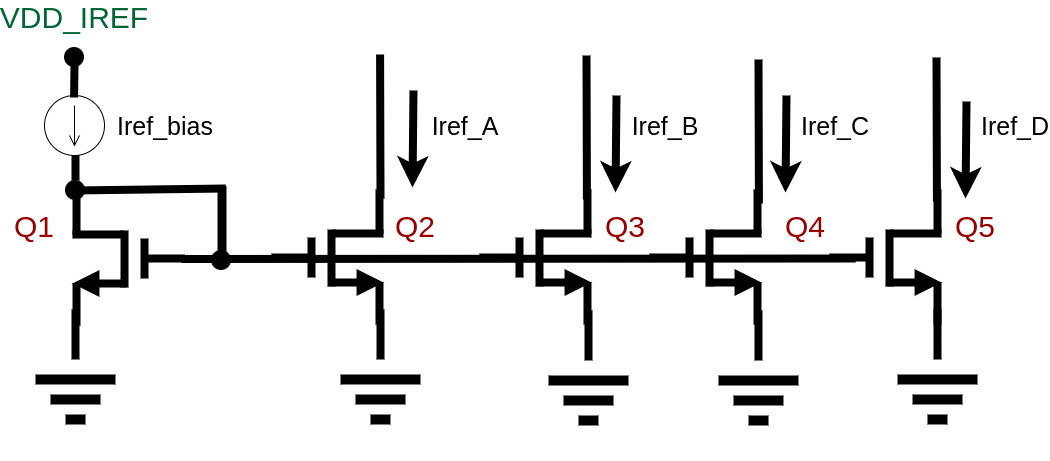
\includegraphics[scale=0.3]{Circuitos/current_mirror.png}
    \legend{Fonte: Produzido pelo autor}
\end{figure}

\begin{figure}[htb]
 \centering
    \centering
    \caption{Representa{\c c}\~ao em bloco do \NomeBloco} \label{\NomeSFig}
    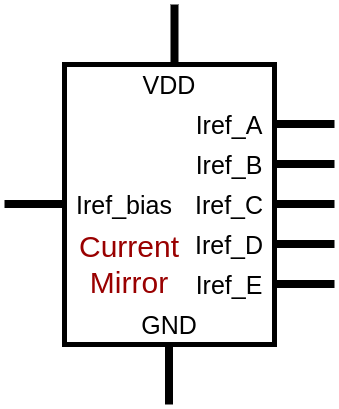
\includegraphics[scale=0.5]{Circuitos/current_mirror_block.png}
    \legend{Fonte: Produzido pelo autor}
\end{figure}

Os transistores utilizados no bloco \NomeBloco{} apresentam os par\^ametros mostrados na \autoref{\NomeTTab}.

\begin{table}[htbp]
\caption{Transistores do Bloco \NomeBloco}
\label{\NomeTTab}
\centering
\begin{tabular}{ccccc}
\toprule
Transistor & W ($\mu$m)  & L ($\mu$m)           & M (n° dispositivos) & S (n° dispositivos)\\
\midrule \midrule
\begin{tabular}[c]{@{}c@{}}Q1, Q2, Q3,\\
Q4, Q5 e Q6\end{tabular} & 5 & 6 & 2 & 1\\
\bottomrule
\end{tabular}
\legend{Fonte: Produzido pelo autor}
\end{table}
\clearpage